%%%%%%%%%%%%%%%%%%%%%%%%%%%%%%%%%%%%%%%%%%%%%%%%%%%%%%%%%%%%%%%%%%%%%%%
%%%%%%%%%%%%%%%%%%%%%%                     %%%%%%%%%%%%%%%%%%%%%%%%%%%%
%%%%%%%%%%%%%%%%%%        End of the book       %%%%%%%%%%%%%%%%%%%%%%%
%%%%%%%%%%%%%%%%%%%%%%                     %%%%%%%%%%%%%%%%%%%%%%%%%%%%
%%%%%%%%%%%%%%%%%%%%%%%%%%%%%%%%%%%%%%%%%%%%%%%%%%%%%%%%%%%%%%%%%%%%%%%
% \begingroup
% \newpage
% \AddToShipoutPicture*{\put(0,0){\includegraphics[width=\paperwidth,height=\paperheight]{back.jpg}}}
% \thispagestyle{empty}

% \begin{center}
%     {\fontsize{20pt}{30pt}\selectfont\color{white}
%         \vspace*{.25\textheight}    
%         \rule{.75\textwidth}{.03cm}
%         \\
%         \vspace*{.75cm}
%         [Fractional Derivatives] will lead to paradox,
%         from which one day useful consequences will be drawn
%         \\
%         \fontsize{10pt}{30pt}\selectfont
%         \textcolor{Golden}{Gottfried Leibniz}
%         \\
%         \vspace*{.75cm}
%         \rule{.75\textwidth}{.03cm}
%     }
% \end{center}
% \endgroup
%%%%%%%%%%%%%%%%%%%%%%%%%%%%%%%%%%%%%%%%%%%%%%%%%%%%%%%%%%%%%%%%%%%%%%%
%%%%%%%%%%%%%%%%%%%%%%                     %%%%%%%%%%%%%%%%%%%%%%%%%%%%
%%%%%%%%%%%%%%%%%%          Other one          %%%%%%%%%%%%%%%%%%%%%%%%
%%%%%%%%%%%%%%%%%%%%%%                     %%%%%%%%%%%%%%%%%%%%%%%%%%%%
%%%%%%%%%%%%%%%%%%%%%%%%%%%%%%%%%%%%%%%%%%%%%%%%%%%%%%%%%%%%%%%%%%%%%%%
\begingroup
\newpage
\AddToShipoutPicture*{\put(0,0){\includegraphics[width=\paperwidth,height=\paperheight]{back.jpg}}}
\thispagestyle{empty}

\begin{figure*}
\vspace*{-2cm}
\hspace*{-1.5cm}
\begin{tikzpicture}[x=0.75pt,y=0.75pt,yscale=-1,xscale=1]
%Image [id:dp12610487456170083] 
\draw (655,140) node  {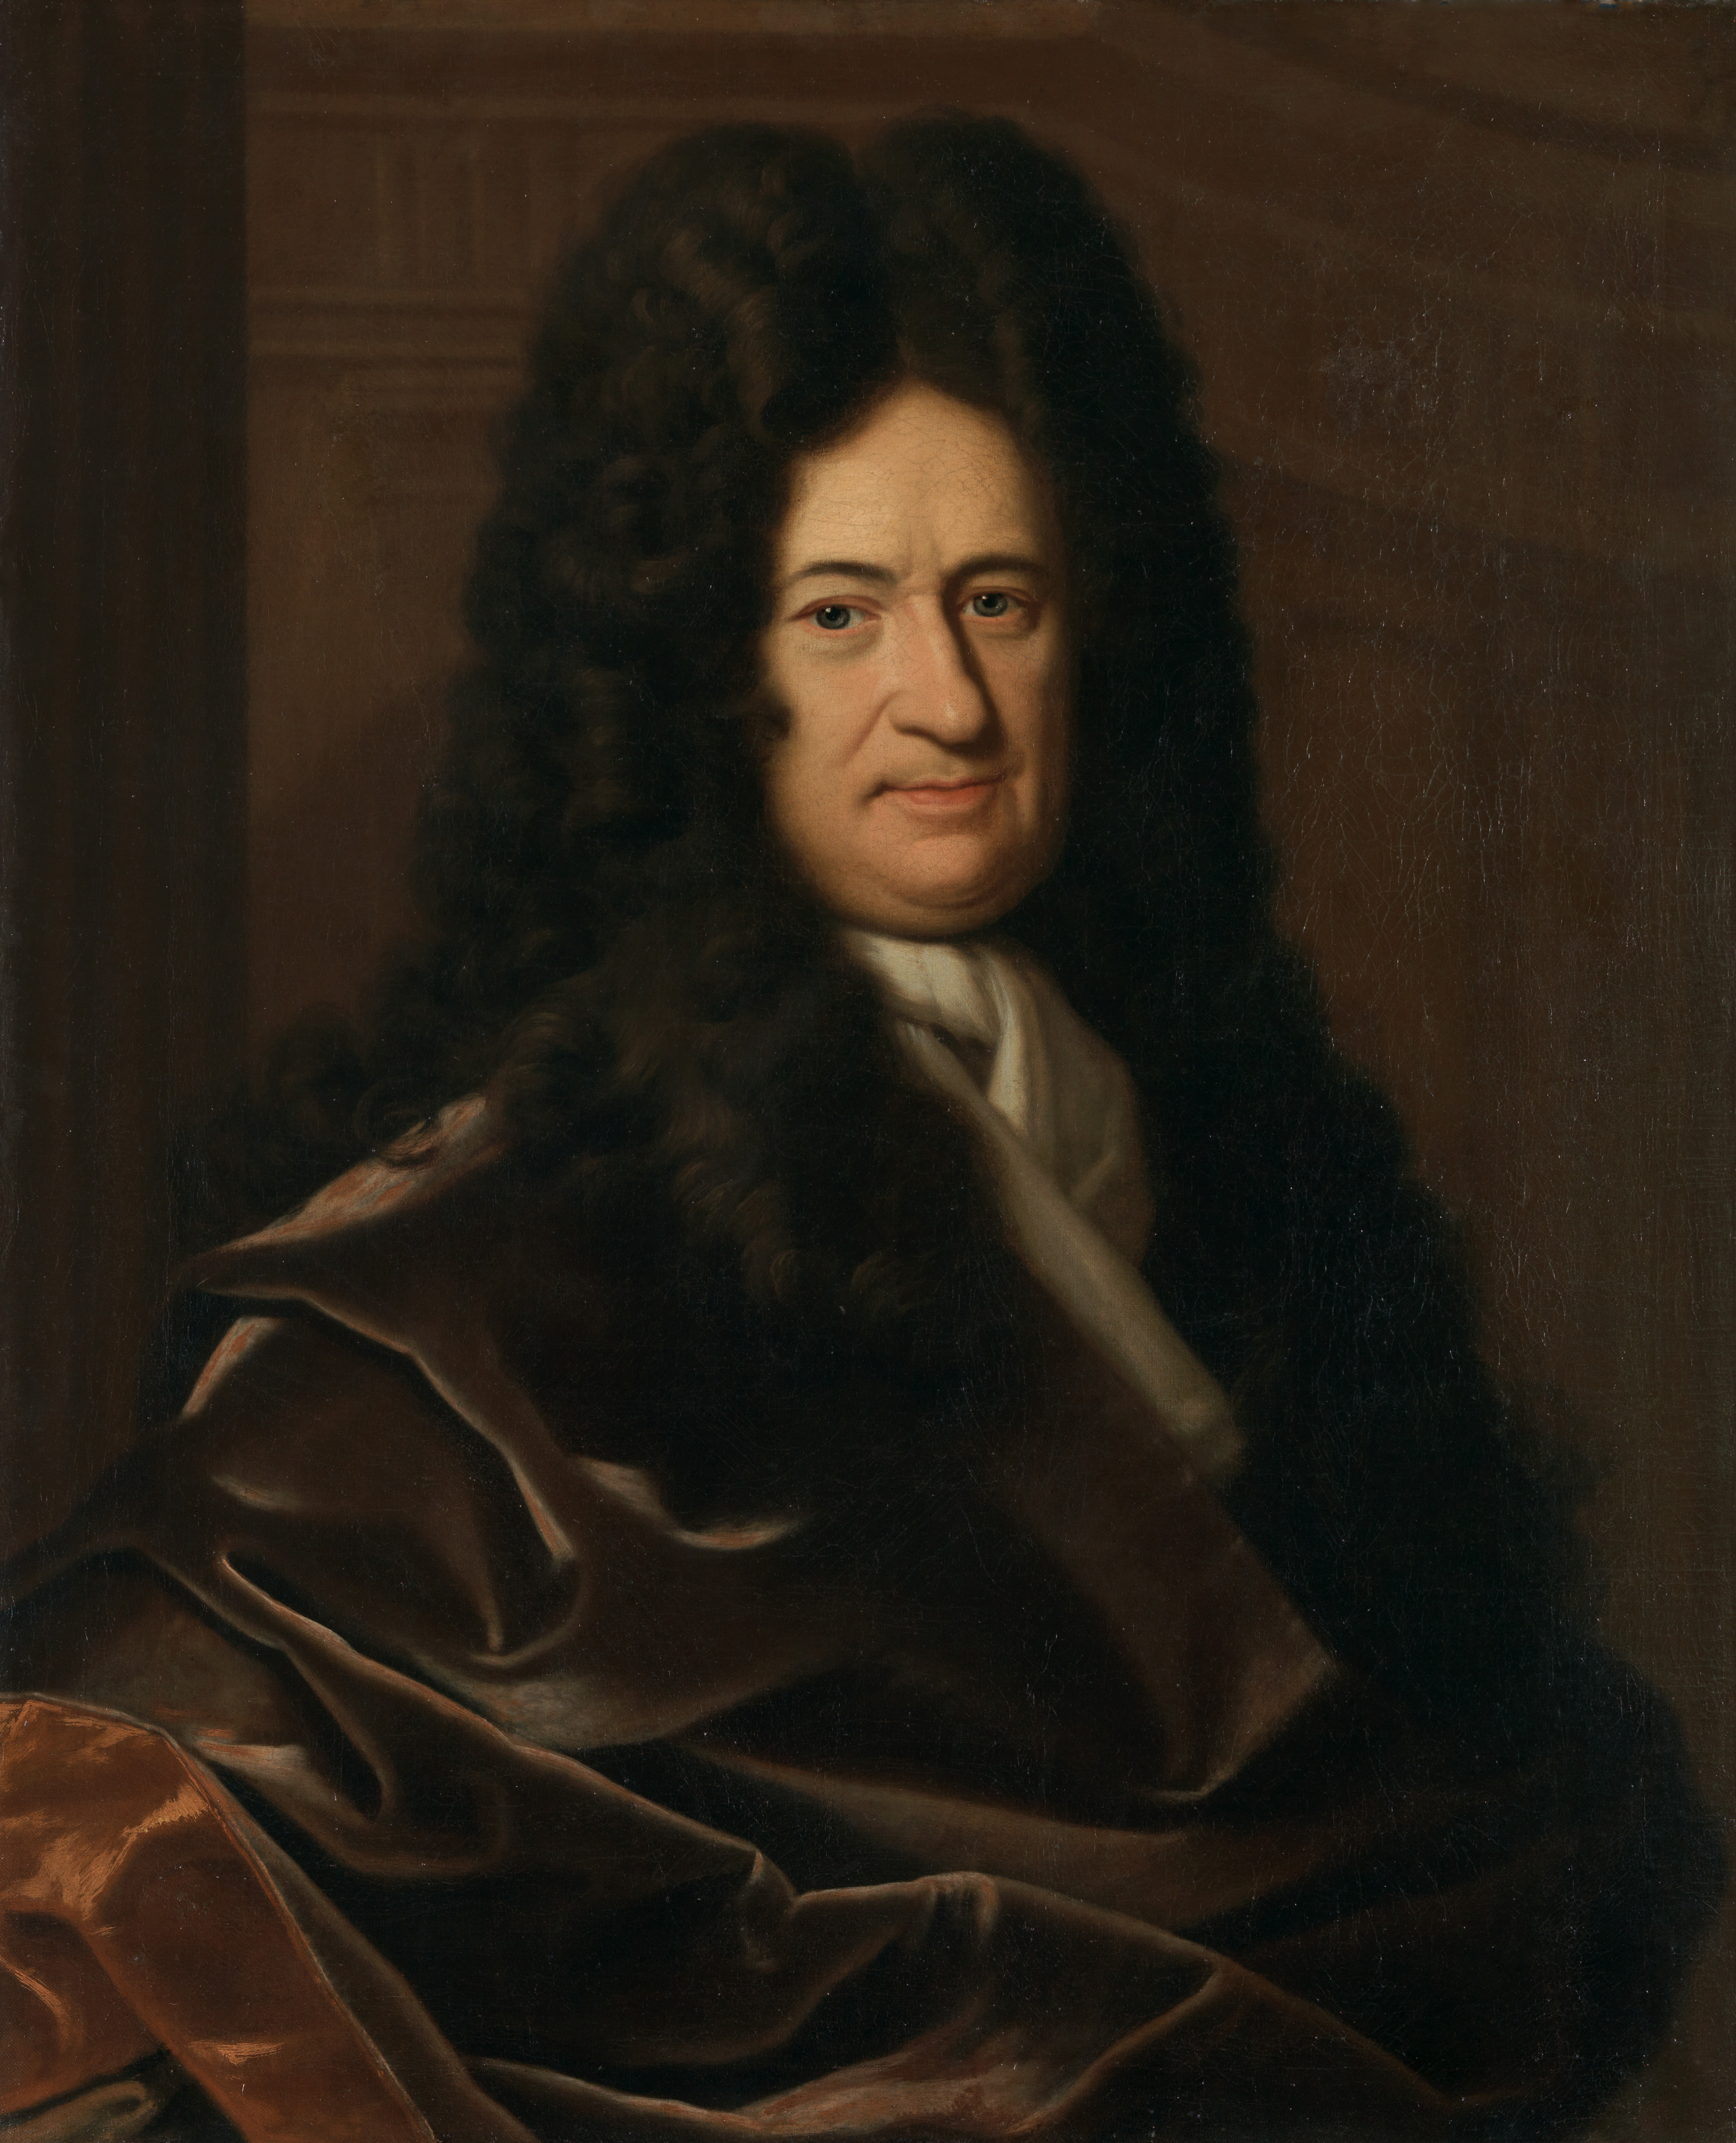
\includegraphics[width=50pt,height=50pt]{Chars/Leibniz.png}};
%Rounded Rect [id:dp5191686460798097] 
\draw  [color={rgb, 255:red, 0; green, 92; blue, 75 }  ,draw opacity=1 ][fill={rgb, 255:red, 0; green, 92; blue, 75 }  ,fill opacity=1 ] (220,156) .. controls (220,147.16) and (227.16,140) .. (236,140) -- (594,140) .. controls (602.84,140) and (610,147.16) .. (610,156) -- (610,204) .. controls (610,212.84) and (602.84,220) .. (594,220) -- (236,220) .. controls (227.16,220) and (220,212.84) .. (220,204) -- cycle ;
%Shape: Half Frame [id:dp24376031746043192] 
\draw  [color={rgb, 255:red, 0; green, 92; blue, 75 }  ,draw opacity=1 ][fill={rgb, 255:red, 0; green, 92; blue, 75 }  ,fill opacity=1 ] (550,140) -- (620,140) -- (599.33,161) -- (571,161) -- (571,189.78) -- (550,211.11) -- cycle ;
%Rounded Rect [id:dp8643336147561154] 
\draw  [color={rgb, 255:red, 54; green, 54; blue, 54 }  ,draw opacity=1 ][fill={rgb, 255:red, 54; green, 54; blue, 54 }  ,fill opacity=1 ] (310,254) .. controls (310,246.27) and (303.73,240) .. (296,240) -- (94,240) .. controls (86.27,240) and (80,246.27) .. (80,254) -- (80,296) .. controls (80,303.73) and (86.27,310) .. (94,310) -- (296,310) .. controls (303.73,310) and (310,303.73) .. (310,296) -- cycle ;
%Shape: Half Frame [id:dp877260980086666] 
\draw  [color={rgb, 255:red, 54; green, 54; blue, 54 }  ,draw opacity=1 ][fill={rgb, 255:red, 54; green, 54; blue, 54 }  ,fill opacity=1 ] (140,240) -- (70,240) -- (91,261) -- (119,261) -- (119,289) -- (140,310) -- cycle ;
%Rounded Rect [id:dp7164157181224868] 
\draw  [color={rgb, 255:red, 54; green, 54; blue, 54 }  ,draw opacity=1 ][fill={rgb, 255:red, 54; green, 54; blue, 54 }  ,fill opacity=1 ] (330,104) .. controls (330,101.79) and (328.21,100) .. (326,100) -- (294,100) .. controls (291.79,100) and (290,101.79) .. (290,104) -- (290,116) .. controls (290,118.21) and (291.79,120) .. (294,120) -- (326,120) .. controls (328.21,120) and (330,118.21) .. (330,116) -- cycle ;
%Rounded Rect [id:dp8914078756100403] 
\draw  [color={rgb, 255:red, 0; green, 92; blue, 75 }  ,draw opacity=1 ][fill={rgb, 255:red, 0; green, 92; blue, 75 }  ,fill opacity=1 ] (220,366) .. controls (220,357.16) and (227.16,350) .. (236,350) -- (594,350) .. controls (602.84,350) and (610,357.16) .. (610,366) -- (610,414) .. controls (610,422.84) and (602.84,430) .. (594,430) -- (236,430) .. controls (227.16,430) and (220,422.84) .. (220,414) -- cycle ;
%Shape: Half Frame [id:dp019193432268682198] 
\draw  [color={rgb, 255:red, 0; green, 92; blue, 75 }  ,draw opacity=1 ][fill={rgb, 255:red, 0; green, 92; blue, 75 }  ,fill opacity=1 ] (550,350) -- (620,350) -- (599.33,371) -- (571,371) -- (571,399.78) -- (550,421.11) -- cycle ;
%Rounded Rect [id:dp21634374173424842] 
\draw  [color={rgb, 255:red, 54; green, 54; blue, 54 }  ,draw opacity=1 ][fill={rgb, 255:red, 54; green, 54; blue, 54 }  ,fill opacity=1 ] (380,324) .. controls (380,321.79) and (378.21,320) .. (376,320) -- (234,320) .. controls (231.79,320) and (230,321.79) .. (230,324) -- (230,336) .. controls (230,338.21) and (231.79,340) .. (234,340) -- (376,340) .. controls (378.21,340) and (380,338.21) .. (380,336) -- cycle ;
%Image [id:dp8518693946864191] 
\draw (35,241.95) node  {\includegraphics[width=50pt,height=50pt]{Chars/lHopital.png}};
%Image [id:dp7198452370903958] 
\draw (655,351.83) node  {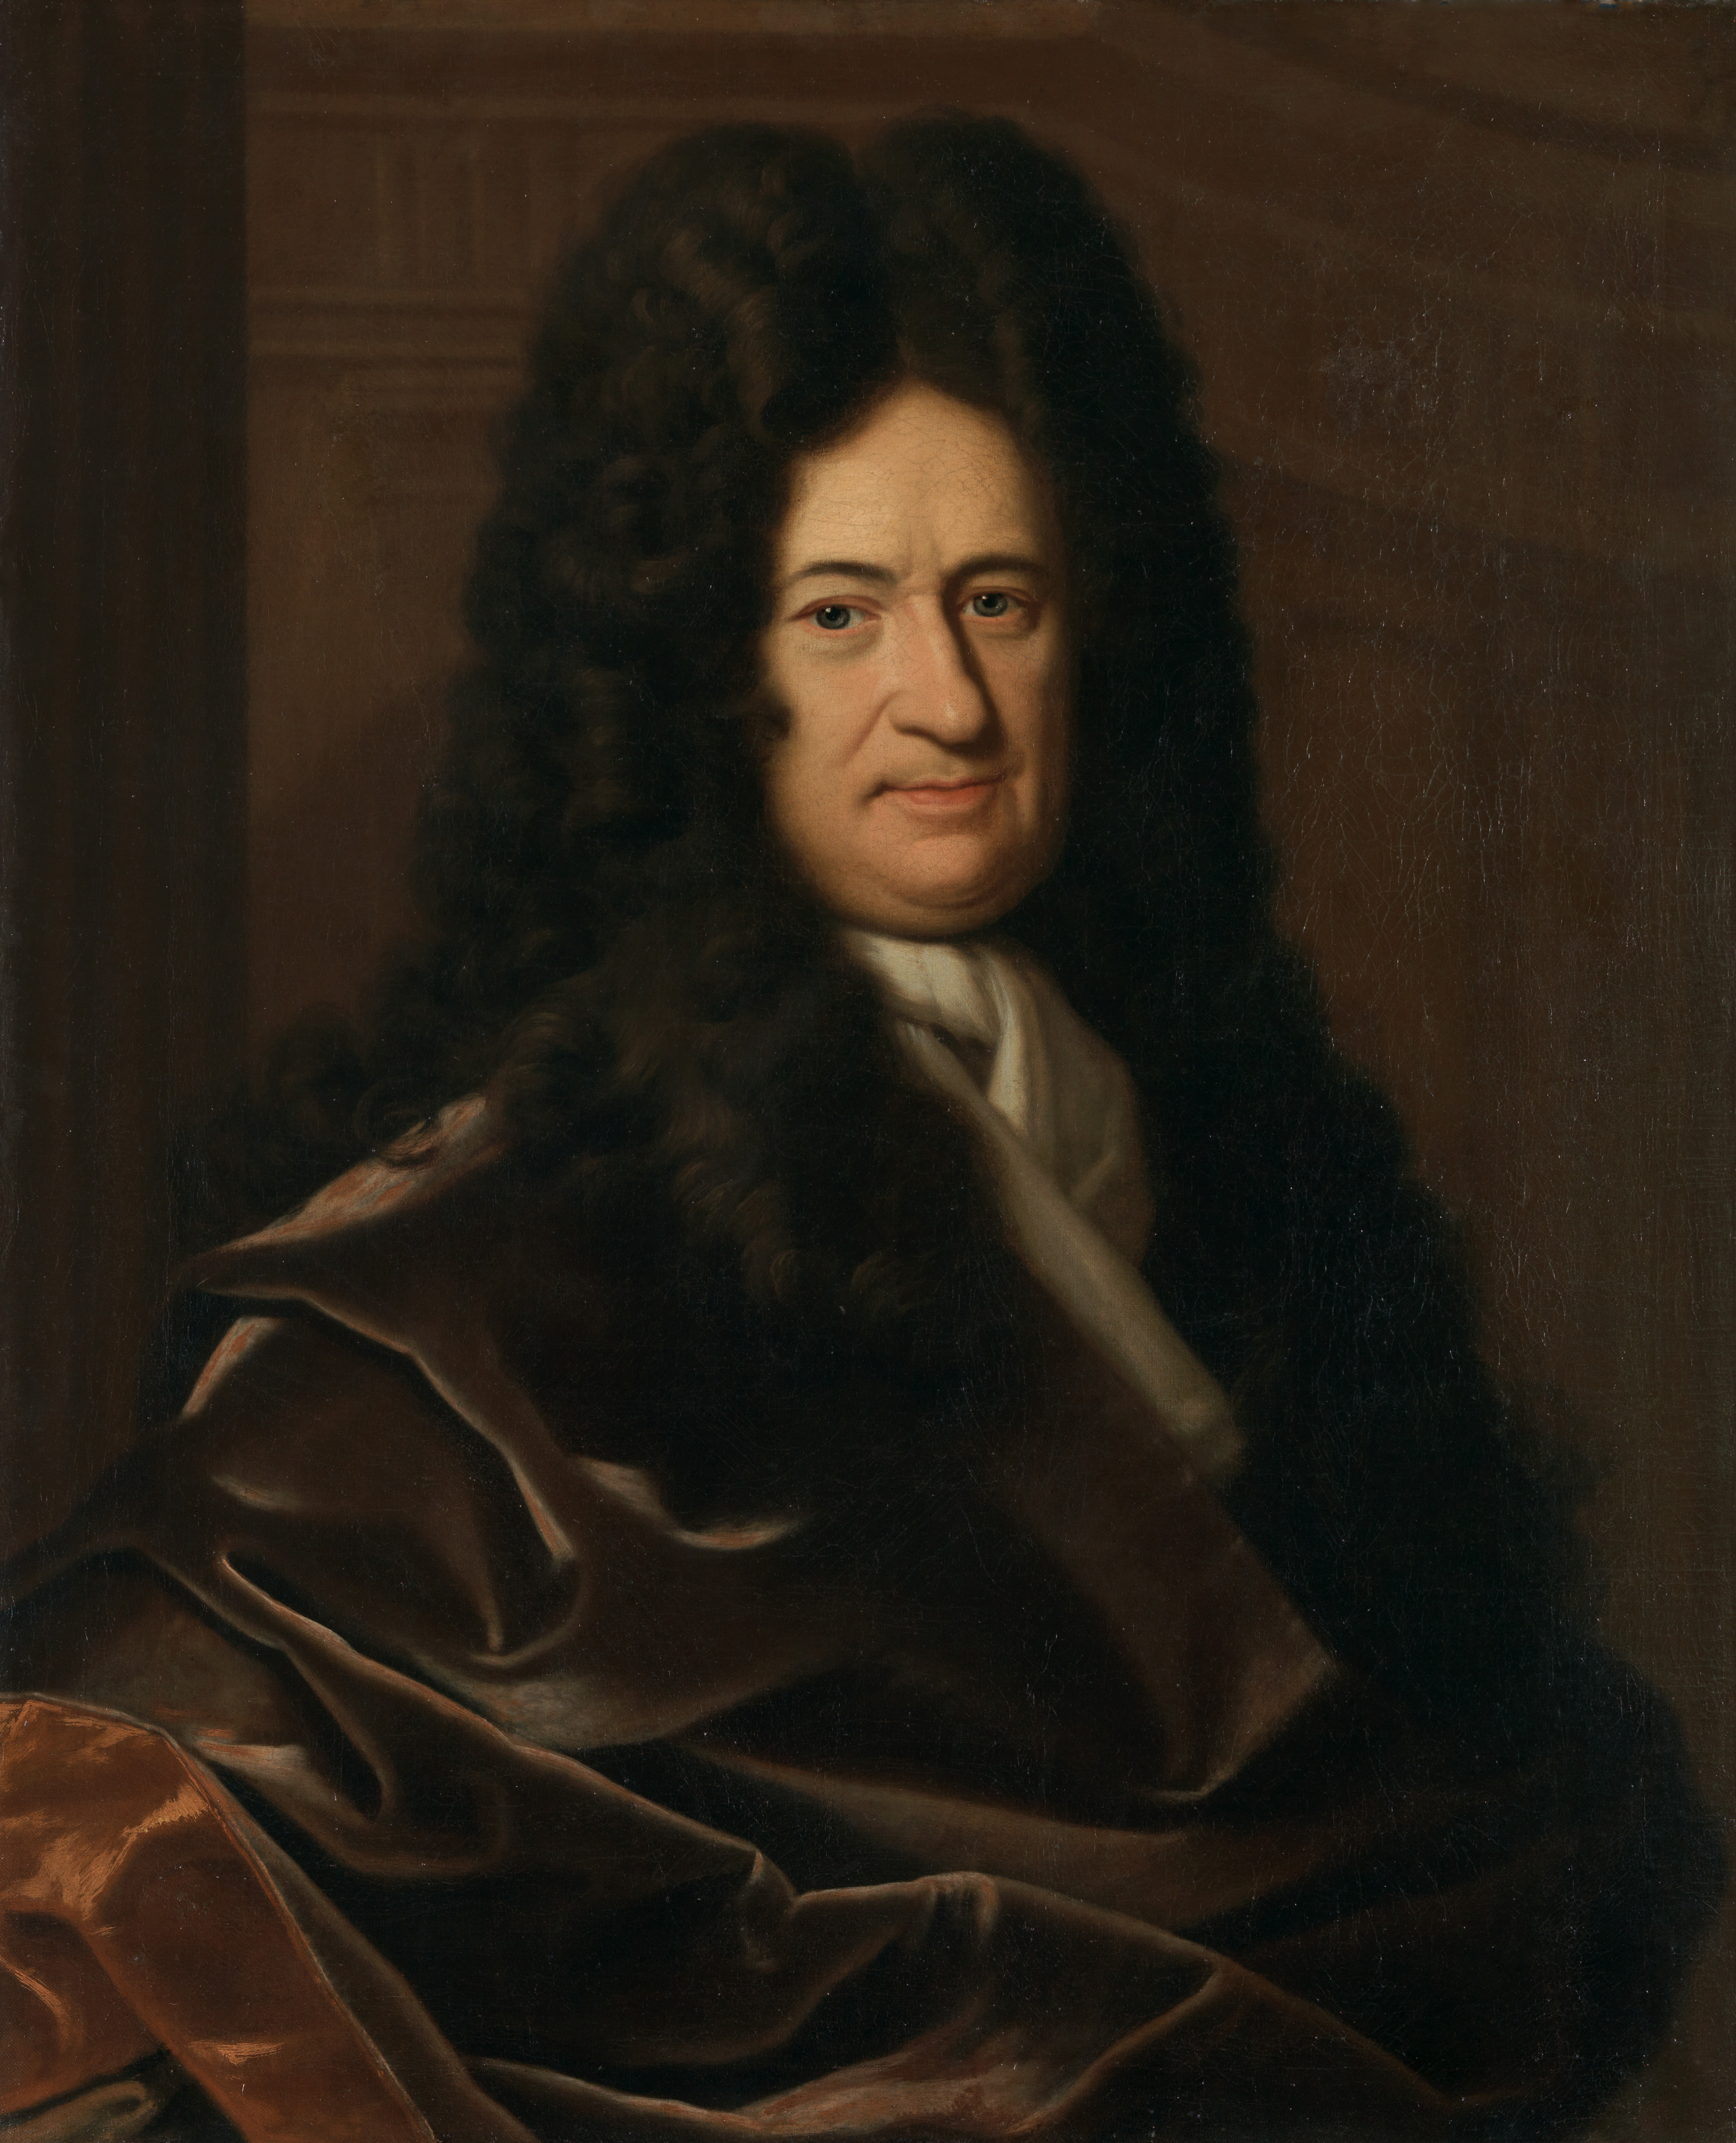
\includegraphics[width=50pt,height=50pt]{Chars/Leibniz.png}};
% Text Node
\draw (231,162.17) node [anchor=north west][inner sep=0.75pt]  [font=\large,color={rgb, 255:red, 252; green, 252; blue, 252 }  ,opacity=1 ] [align=left] {Can the meaning of derivative with integer order be \\generalized to derivative with non-integer order?!};
% Text Node
\draw (91,257.75) node [anchor=north west][inner sep=0.75pt]  [font=\large,color={rgb, 255:red, 252; green, 252; blue, 252 }  ,opacity=1 ] [align=left] {What if the order will be $\displaystyle \frac{1}{2}$?!};

% Text Node
\draw (552,143) node [anchor=north west][inner sep=0.75pt]  [color={rgb, 255:red, 255; green, 215; blue, 0 }  ,opacity=1 ] [align=left] {Leibniz};
% Text Node
\draw (94,244.83) node [anchor=north west][inner sep=0.75pt]  [color={rgb, 255:red, 255; green, 215; blue, 0 }  ,opacity=1 ] [align=left] {L'Hopital};
% Text Node
\draw (581,202) node [anchor=north west][inner sep=0.75pt]  [color={rgb, 255:red, 57; green, 159; blue, 185 }  ,opacity=1 ] [align=left] {$\surd$};
% Text Node
\draw (584,202) node [anchor=north west][inner sep=0.75pt]  [color={rgb, 255:red, 57; green, 159; blue, 185 }  ,opacity=1 ] [align=left] {$\surd$};
% Text Node
\draw (291,102) node [anchor=north west][inner sep=0.75pt]  [font=\large , color={rgb, 255:red, 254; green, 254; blue, 254 }  ,opacity=1 ] [align=left] {1695};
% Text Node
\draw (91,292) node [anchor=north west][inner sep=0.75pt]  [color={rgb, 255:red, 57; green, 159; blue, 185 }  ,opacity=1 ] [align=left] {$\surd$};
% Text Node
\draw (94,292) node [anchor=north west][inner sep=0.75pt]  [color={rgb, 255:red, 57; green, 159; blue, 185 }  ,opacity=1 ] [align=left] {$\surd$};
% Text Node
\draw (231,372.17) node [anchor=north west][inner sep=0.75pt]  [font=\large , color={rgb, 255:red, 252; green, 252; blue, 252 }  ,opacity=1 ] [align=left] {It will lead to a paradox, from which one day useful \\consequences will be drawn};
% Text Node
\draw (581,412) node [anchor=north west][inner sep=0.75pt]  [color={rgb, 255:red, 57; green, 159; blue, 185 }  ,opacity=1 ] [align=left] {$\surd$};
% Text Node
\draw (584,412) node [anchor=north west][inner sep=0.75pt]  [color={rgb, 255:red, 57; green, 159; blue, 185 }  ,opacity=1 ] [align=left] {$\surd$};
% Text Node
\draw (236,323) node [anchor=north west][inner sep=0.75pt]  [font=\large , color={rgb, 255:red, 254; green, 254; blue, 254 }  ,opacity=1 ] [align=left] {September 30, 1695};
% Text Node
\draw (551,352) node [anchor=north west][inner sep=0.75pt]  [color={rgb, 255:red, 255; green, 215; blue, 0 }  ,opacity=1 ] [align=left] {Leibniz};
\end{tikzpicture}
\end{figure*}
\endgroup











